\section[1997年高考数学试卷及答案(全国卷)理科]{1997年普通高等学校招生考试(全国卷)\\\Huge{理科数字}}

\begin{questions}
	\question 设集合$M=\{x|0 \leqslant x < 2\}$,集合$N=\{x|x^2 - 2x - 3 <0\}$,集合$M\cap N=$ \hfill (\hspace{2cm})
	\begin{oneparchoices}
		\choice $\{x|0\leqslant x < 1\}$
		\CorrectChoice $\{x|0\leqslant x < 2\}$
		\choice $\{x|0\leqslant x \leqslant 1\}$
		\choice $\{x|0\leqslant x \leqslant 2\}$
	\end{oneparchoices}

	\begin{solution}
		集合$N=\{x|-1 < x < 3\}$,两个集合的范围如下图所示:

		\begin{tikzpicture}
			\tkzInit[xmin=-4, xmax=4]
			\tkzDrawX

			\draw[rounded corners=2pt, thick, black!50] (-1,0) |- (3,.5) -- (3,0);
			\draw[black!50, thick, pattern=north east lines,pattern color=black!50, rounded corners=2pt] (0,0) |- (2,.8) -- (2,0);
			\draw [fill=white](-1,0) circle (1pt);
			\draw [fill=white](3,0) circle (1pt);
			\draw [fill=black](0,0) circle (1pt);
			\draw [fill=white](2,0) circle (1pt);
		\end{tikzpicture}
	\end{solution}

	\question 如果直线$ax+2y+2=0$与直线$3x-y-2=0$平行,那么系数$a=$ \hfs

	\begin{oneparchoices}
		\choice $-3$
		\CorrectChoice $-6$
		\choice $-\dfrac32$
		\choice $\dfrac23$
	\end{oneparchoices}

	\begin{solution}
		两条直线平行则其斜率相等,可得:
		\begin{equation*}
			-\frac{a}{2} = 3
		\end{equation*}
		所以答案为$a=-6$
	\end{solution}

	\question 函数$y=\tan \left( \dfrac12x - \dfrac{\pi}{3} \right)$在一个周期内的图像是 \hfs

	\begin{oneparchoices}
		\pgfplotsset{
			xlabel={$x$},
			ylabel={$y$},
			% x label style={at={(current axis.right of origin)}, anchor=north},
			axis lines=center,
			samples=100,
			ticks=none
		}
		\CorrectChoice
		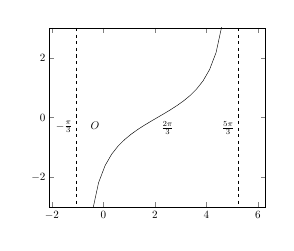
\begin{tikzpicture}[scale=.4]
			\begin{axis}[
					xmin = {-2/3*pi},
					xmax = {2*pi},
					ymin = -3,
					ymax = 3,
				]
				\addplot[domain={-1/3*pi+0.1}:{5/3*pi-0.1}]{tan(deg(1/2*x - pi/3))};
				\draw[dashed] (-pi/3,3) -- (-pi/3, -3);
				\draw[dashed] (pi*5/3,3) -- (pi*5/3, -3);
				\node[below left] at (-pi/3, 0) {$-\frac{\pi}{3}$};
				\node[below right] at (2*pi/3, 0) {$\frac{2\pi}{3}$};
				\node[below left] at (5*pi/3, 0) {$\frac{5\pi}{3}$};
				\node[below left] at (0,0) {$O$};
			\end{axis}
		\end{tikzpicture}
		\choice
		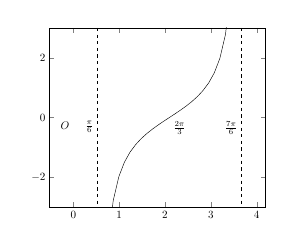
\begin{tikzpicture}[scale=.4]
			\begin{axis}[
					xmin = {-1/6*pi},
					xmax = {8/6*pi},
					ymin = -3,
					ymax = 3,
				]
				\addplot[domain={1/6*pi+0.1}:{7/6*pi-0.1}]{tan(deg(x - 2/3*pi))};
				\draw[dashed] (pi/6,3) -- (pi/6, -3);
				\draw[dashed] (pi*7/6,3) -- (pi*7/6, -3);
				\node[below left] at (pi/6, 0) {$\frac{\pi}{6}$};
				\node[below right] at (2*pi/3, 0) {$\frac{2\pi}{3}$};
				\node[below left] at (7*pi/6, 0) {$\frac{7\pi}{6}$};
				\node[below left] at (0,0) {$O$};
			\end{axis}
		\end{tikzpicture}
		\choice
		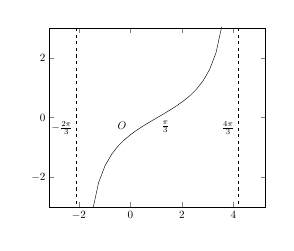
\begin{tikzpicture}[scale=.4]
			\begin{axis}[
					xmin = {-pi},
					xmax = {5/3*pi},
					ymin = -3,
					ymax = 3,
				]
				\addplot[domain={-2/3*pi+0.1}:{4/3*pi-0.1}]{tan(deg(1/2*x - pi/6))};
				\draw[dashed] (-pi*2/3,3) -- (-pi*2/3, -3);
				\draw[dashed] (pi*4/3,3) -- (pi*4/3, -3);
				\node[below left] at (-pi*2/3, 0) {$-\frac{2\pi}{3}$};
				\node[below right] at (pi/3, 0) {$\frac{\pi}{3}$};
				\node[below left] at (4*pi/3, 0) {$\frac{4\pi}{3}$};
				\node[below left] at (0,0) {$O$};
			\end{axis}
		\end{tikzpicture}
		\choice
		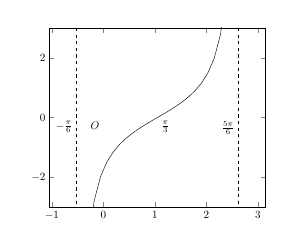
\begin{tikzpicture}[scale=.4]
			\begin{axis}[
					xmin = {-1/3*pi},
					xmax = {pi},
					ymin = -3,
					ymax = 3,
				]
				\addplot[domain={-1/6*pi+0.1}:{5/6*pi-0.1}]{tan(deg(x - 1/3*pi))};
				\draw[dashed] (-pi/6,3) -- (-pi/6, -3);
				\draw[dashed] (pi*5/6,3) -- (pi*5/6, -3);
				\node[below left] at (-pi/6, 0) {$-\frac{\pi}{6}$};
				\node[below right] at (pi/3, 0) {$\frac{\pi}{3}$};
				\node[below left] at (5*pi/6, 0) {$\frac{5\pi}{6}$};
				\node[below left] at (0,0) {$O$};
			\end{axis}
		\end{tikzpicture}
	\end{oneparchoices}
	\begin{solution}
		$\tan{x}$的周期是$\pi$,所以$\tan{\frac12{x}}$的周期应该为$2\pi$.因此排除B和D.
		$\tan(\frac12\cdot\frac{\pi}{3}-\frac{\pi}{3}) \neq 0$,因此选A.
	\end{solution}
	\question
	已知三棱锥$D-ABC$的三个侧面与底面全等,且$AB=AC=\sqrt{3}$,$BC=2$,则以$BC$为棱,以面$BCD$与面$BCA$为面的二面角的大小是
	\hfs

	\begin{oneparchoices}
		\choice $\arccos\dfrac{\sqrt{3}}{3}$
		\choice $\arccos\dfrac{1}{3}$
		\CorrectChoice $\dfrac{\pi}{2}$
		\choice $\dfrac{2\pi}{3}$
	\end{oneparchoices}
	\pagebreak
	\begin{solution}

		\tdplotsetmaincoords{20}{120}
		\begin{center}
			\begin{tikzpicture}[tdplot_main_coords, baseline=(current bounding box.north), scale=1.5]
				\coordinate(A) at ({sqrt(2)}, 0);
				\coordinate(B) at (0,1);
				\coordinate(C) at (0,-1);
				\coordinate(D) at (0,0,{sqrt(2)});

				\draw(A)node[below]{$A$} -- (B)node[below]{$B$};
				\draw[dashed](B)-- (C)node[above]{$C$};
				\draw(C)-- (A);
				\draw(D)node[above]{$D$} -- (A);
				\draw(D) -- (B);
				\draw(D) -- (C);

				\draw[blue, dashed](A) -- (0,0)node[below right]{$O$} -- (D);
			\end{tikzpicture}
		\end{center}

		取$BC$的中点为$O$,连接$AO$和$DO$.
		因为$AC=AB$,所以有$AO\perp BC$.因为$\triangle{BCD}\cong\triangle{BCA}$,所以也有$DO\perp
			BC$.计算可得$AO=DO=\sqrt{2}$.另外有$AD=2$.可以看出有$AO^2 + DO^2 =
			AD^2$,所以$\triangle{AOD}$是直角三角形,即二面角为$\ang{90}$.
	\end{solution}

	\question 函数$y=\sin \left( \dfrac{\pi}{3} - 2x \right) + \cos2x$的最小正周期是 \hfs

	\begin{oneparchoices}
		\choice $\dfrac{\pi}{2}$
		\CorrectChoice $\pi$
		\choice $2\pi$
		\choice $\dfrac{2\pi}{3}$
	\end{oneparchoices}

	\begin{solution}
		因为$\sin \left( \dfrac{\pi}{3} -2x \right)$与$\cos2x$的周期均为$\pi$,所以函数的最小正周期也为$\pi$.
	\end{solution}

	\question 满足$\arccos(1-x) \geqslant \arccos{x}$的取值范围是 \hfs

	\begin{oneparchoices}
		\choice $\left[-1, -\dfrac12\right]$
		\choice $\left[-\dfrac12, 0\right]$
		\choice $\left[0, \dfrac12\right]$
		\CorrectChoice $\left[\dfrac12, 1\right]$
	\end{oneparchoices}

	\begin{solution}
		因为$\arccos$的定义域是$[-1,1]$,所以排队选项A和B.

		$\arccos(0) = \frac{\pi}{2}, \arccos(1-0)=0$,所以C也可以排除.答案为D.
	\end{solution}

	\question 将$y=2^x$的图像\underline{\hspace{.5cm}},再作关于直线$y=x$对称的图像,可得到函数$y=\log_2(x+1)$的图像. \hfs

	\begin{oneparchoices}
		\choice 先向左平移$1$个单位
		\choice 先向右平移$1$个单位
		\choice 先向上平移$1$个单位
		\CorrectChoice 先向下平移$1$个单位
	\end{oneparchoices}

	\begin{solution}
		点$(0,0)$在直线$y=x$上,并且也在函数$y=\log_2(x+1)$上,所以应该也在$y=2^x$平移后的图像上,可以得到平移后的图像为$y=2^x
			- 1$才能满足点$(0,0)$在图像上.
	\end{solution}

	\question 长方体一个顶点上三条棱的长分别是$3,4,5$,且它的八个顶点都在同一个球面上,这个球的表面积是

	\hfs

	\begin{oneparchoices}
		\choice $20\sqrt{2}\pi$
		\choice $25\sqrt{2}\pi$
		\CorrectChoice $50\pi$
		\choice $200\pi$
	\end{oneparchoices}
	\pagebreak
	\begin{solution}
		\tdplotsetmaincoords{60}{120}
		\begin{center}
			\begin{tikzpicture}[tdplot_main_coords]
				\coordinate (A) at (0,0);
				\coordinate (B) at (3,0);
				\coordinate (C) at (3,4);
				\coordinate (D) at (0,4);
				\coordinate (A') at (0,0,5);
				\coordinate (B') at (3,0,5);
				\coordinate (C') at (3,4,5);
				\coordinate (D') at (0,4,5);

				\draw (B) -- (C) -- (D);
				\draw[dashed] (A) -- (B) (D) -- (A);
				\draw (A') -- (B') -- (C') -- (D') -- cycle;
				\draw[dashed] (A) -- (A');
				\draw (B) -- (B');
				\draw (C) -- (C');
				\draw (D) -- (D');
				\draw[dashed] (A) -- (C');
				\draw[dashed] (A) -- (C);

				\tkzLabelPoint[left](A){$A$}
				\tkzLabelPoint[left](B){$B$}
				\tkzLabelPoint[below](C){$C$}
				\tkzLabelPoint[above](C'){$C'$}
			\end{tikzpicture}
		\end{center}

		\begin{align*}
			AB = 3, BC = 4, CC'= 5             \\
			AC = \sqrt{3^2 + 4^2} = 5          \\
			AC' = \sqrt{5^2 + 5^2} = 5\sqrt{2} \\
		\end{align*}
		则球体的半径为$\frac12AC'=\frac{5\sqrt{2}}{2}$, 球体的表面积为$4\pi \left( \frac{5\sqrt{2}}{2} \right)^2=50\pi$.
	\end{solution}

	\question 曲线的参数方程是\begin{math}
		\begin{cases}
			x = 1 - \dfrac1t \\
			y = 1 - t^2
		\end{cases}(t是参数,t\neq0),它的普通方程是 \hfs
	\end{math}

	\begin{oneparchoices}
		\choice $(x-1)^2(y-1)=1$
		\CorrectChoice $y=\dfrac{x(x-2)}{(1-x)^2}$
		\choice $y=\dfrac{1}{(1-x)^2} -1$
		\choice $y=\dfrac{x}{1-x^2} + 1$
	\end{oneparchoices}

	\begin{solution}
		由$x = 1 - \dfrac1t$得$t=\dfrac{1}{1-x}$,代入$y=1-t^2$得
		\begin{align*}
			y & = 1- \frac{1}{(1-x)^2}           \\
			  & = \frac{1-2x + x^2 - 1}{(1-x)^2} \\
			  & = \frac{x(x-2)}{(1-x)^2}
		\end{align*}
	\end{solution}

	\question 函数$y=\cos^2x-3\cos{x} + 2$的最小值为 \hfs

	\begin{oneparchoices}
		\choice $2$
		\CorrectChoice $0$
		\choice $-\dfrac14$
		\choice $6$
	\end{oneparchoices}

	\begin{solution}
		\begin{align*}
			y & = \cos^2x - 3x + \frac94 - \frac14 \\
			  & = (\cos{x} - \frac32)^2 - \frac14  \\
		\end{align*}
		$(\cos{x}-\dfrac32)^2$最小值为$\dfrac14$,则函数的最小值为$0$.
	\end{solution}

	\question 椭圆$C$与椭圆$\dfrac{(x-3)^2}{9} + \dfrac{(y-2)^2}{4}=1$关于直线$x+y=0$对称,椭圆$C$的方程是 \hfs

	\begin{choices}
		\CorrectChoice $\dfrac{(x+2)^2}{4} + \dfrac{(y+3)^2}{9} = 1$
		\choice $\dfrac{(x-2)^2}{9} + \dfrac{(y-3)^2}{4} = 1$
		\choice $\dfrac{(x+2)^2}{9} + \dfrac{(y+3)^2}{4} = 1$
		\choice $\dfrac{(x-2)^2}{4} + \dfrac{(y-3)^2}{9} = 1$
	\end{choices}

	\begin{solution}
		对于椭圆$C$上的任一点$(x,y)$,其关于直线$x+y=0$对称的点为$(-y, -x)$,代入椭圆方程得:
		\begin{align*}
			\frac{(-y-3)^2}{9} + \frac{(-x-2)^2}{4} & = 1 \\
			\frac{(y+3)^2}{9} + \frac{(x+2)^2}{4}   & = 1
		\end{align*}
	\end{solution}

	\question 圆台上、下底面积分别为$\pi$、$4\pi$,侧面积为$6\pi$,这个圆台的体积是\hfs

	\begin{oneparchoices}
		\choice $\dfrac{2\sqrt{3}\pi}{3}$
		\choice $2\sqrt{3}\pi$
		\choice $\dfrac{7\sqrt{3}\pi}{6}$
		\CorrectChoice $\dfrac{7\sqrt{3}\pi}{3}$
	\end{oneparchoices}

	\begin{solution}
		\tdplotsetmaincoords{80}{0}
		\begin{center}
			\begin{tikzpicture}[tdplot_main_coords]
				\draw[dashed] (2,0) arc (0:180:2);
				\draw (2,0) arc (0:-180:2);
				\draw (0,0,1) circle(1);

				\draw[thin] (2,0,0) -- node[above, sloped]{$l$}(1,0,1);
				\draw[thin] (-2,0,0) -- (-1,0,1);

				\draw (0,0,1)node[left]{$r_2$} -- (1,0,1);
				\draw[dashed] (0,0)node[left]{$r_1$} -- (2,0);
				\draw[dashed] (0,0) -- (0,0,2);
				\draw[dashed] (0,0,2) --node[above, sloped]{$l'$} (1,0,1);
			\end{tikzpicture}
		\end{center}

		圆台的侧面积$=\pi(l+l')r_1 - \pi l'r_2$,而$\frac{l'}{l'+l}=\frac{r_2}{r_1}=\frac12$,即$l'=l$,代入面积公式中得:
		$3\pi l = 6\pi$,得到$l=2$.圆台的高$h=\sqrt{l^2-(r_1-r_2)^2}=\sqrt{3}$.
		\begin{align*}
			V & = \frac13h{(S_上 + S_下 + \sqrt{S_上S_下})} \\
			  & = \frac{7\sqrt{3}\pi}{3}
		\end{align*}
	\end{solution}

	\question
	定义在区间$(-\infty,+\infty)$的奇函数$f(x)$为增函数,偶函数$g(x)$在区间$[0,+\infty)$的图像与$f(x)$的图像重合,设$a>b>0$,给出下列不等式:

	\circled{1}$f(b)-f(-a)>g(a)-g(-b)$; \circled{2}$f(b)-f(-a) < g(a) - g(-b)$;
	\circled{3}$f(a)-f(-b) > g(b) - g(-a)$; \circled{4}$f(a)-f(-b) < g(b) - g(-a)$.
	其中成立的是 \hfs

	\begin{oneparchoices}
		\choice \circled{1}与\circled{4}
		\choice \circled{2}与\circled{3}
		\CorrectChoice \circled{1}与\circled{3}
		\choice \circled{2}与\circled{4}
	\end{oneparchoices}

	\begin{solution}
		\begin{enumerate}[label=\protect\circled{\arabic*}]
			\item $f(b) - f(-a) = f(b)+f(a)$, $g(a) - g(-b) = g(a) - g(b)$,所以有$f(b)-f(-a) > g(a) - g(-b)$;
			\item 不成立;
			\item $f(a) - f(-b) = f(a) + f(b)$, $g(b) - g(-a)= g(b) - g(a)$,所以有$f(a) - f(-b) > g(b) - g(-a)$
			\item 不成立
		\end{enumerate}
	\end{solution}

	\question 不等式组 \begin{math}
		\begin{cases}
			x> 0 \\
			\dfrac{3-x}{3+x} > \left|\dfrac{2-x}{2+x}\right|
		\end{cases}
	\end{math}的解集是 \hfs

	\begin{oneparchoices}
		\choice $\{x|0< x < 2\}$
		\choice $\{x|0< x < 2.5\}$
		\CorrectChoice $\{x|0< x < \sqrt{6}\}$
		\choice $\{x|0< x < 3\}$
	\end{oneparchoices}

	\begin{solution}
		从\begin{math}
			\begin{cases}
				x> 0 \\
				\dfrac{3-x}{3+x} > \left|\dfrac{2-x}{2+x}\right|
			\end{cases}
		\end{math}可得
		\begin{align*}
			\frac{3-x}{3+x} & > \frac{2-x}{2+x} \qquad (-2 < x \leqslant 2) \tag{1}          \\
			\frac{3-x}{3+x} & > \frac{x-2}{2+x}  \qquad (-2 > x(x\neq-3) \cup x > 2) \tag{2}
		\end{align*}
		由式$(1)$得
		\begin{align*}
			6+x-x^2> 6-x -x^2 \qquad (-2 \leqslant x \leqslant 2) \\
			0 < x \leqslant 2 \tag{a}
		\end{align*}
		由式$(2)$得
		\begin{align*}
			6 +x - x^2 > -6 +x + x^2 \qquad (-2 > x(x\neq-3) \cup x > 2) \\
			6 > x^2 \qquad (-2 > x (x\neq-3) \cup x > 2)                 \\
			-\sqrt{6} < x < -2, 2 < x < \sqrt{6} \tag{b}
		\end{align*}
		综合$(a)$和$(b)$可得 $-\sqrt{6}<x < -2, 0< x <
			\sqrt{6}$,再结合题目中$x>0$的条件,所以最后的解集是$\{x|0<x<\sqrt{6}\}$
	\end{solution}

	\question 四面体的顶点和各棱中点共$10$个点,在其中取$4$个不共面的点,不同的取法共有 \hfs

	\begin{oneparchoices}
		\choice $150$种
		\choice $147$种
		\choice $144$种
		\CorrectChoice $141$种
	\end{oneparchoices}

	\begin{solution}
		\begin{enumerate}[label=\protect\circled{\arabic*}]
			\item 从$10$个点中取$4$个点一共有$\binom{10}{4}=\frac{10\times9\times8\times7}{4\times3\times2\times1}=210$种.
			\item 四面体上一个面上有规定的$6$个点,从这$6$个点中取$4$个点的取法有$\binom{6}{4}=15$种,一共有$4$个面,所以取得在同一个面上的$4$个点的取法有$60$种.
			\item 下面考虑不是现有的四个面上但是也在一个平面的情况:
			      \begin{enumerate}[label=\Roman*]
				      \item 一条棱边上的三个点与其对面的棱的中点所成的平面,这种情况有6种(棱边有6条);
				      \item 一个侧面的两个侧棱中点的连线与底面中对应的两条棱边中点连线是平行的,因为也共面.这样的情况有三种.
				            \begin{center}
					            \tdplotsetmaincoords{60}{120}
					            \begin{tikzpicture}[tdplot_main_coords]
						            \coordinate(A) at (0,0);
						            \coordinate(C') at (1.5,0);
						            \coordinate(B) at (3,0);
						            \coordinate(B') at (1.5, 2);
						            \coordinate(C) at (0,4);
						            \coordinate(A') at (0,2);
						            \coordinate(D) at (2,2,5);

						            \coordinate(D1) at ($(D)!0.5!(A)$);
						            \coordinate(D2) at ($(D)!0.5!(B)$);
						            \coordinate(D3) at ($(D)!0.5!(C)$);

						            \draw[dashed] (A) -- (B) (A) -- (C) (D) -- (A);
						            \draw[dashed, red](D2) --  (C') -- (A')--(D3) (B) -- (D1) -- (C);
						            \draw[dashed, blue](B) -- (D1) -- (C);
						            \draw (D) -- (B) (D) -- (C) (B) -- (C) (D2) -- (C) (D2) -- (D3);
						            \tkzLabelPoint(A){$A$}
						            \tkzLabelPoint(B){$B$}
						            \tkzLabelPoint(C){$C$}
						            \tkzLabelPoint[right](D1){$D_1$}
						            \tkzLabelPoint[left](D2){$D_2$}
						            \tkzLabelPoint[right](D3){$D_3$}
						            \tkzLabelPoint[above, sloped](A'){$A'$}
						            \tkzLabelPoint(B'){$B'$}
						            \tkzLabelPoint[above, sloped](C'){$C'$}
						            \tkzDrawPoints[color=blue, fill=blue](A',B',C',D1,D2,D3)
						            \tkzLabelPoint[above](D){$D$}

					            \end{tikzpicture}
				            \end{center}
			      \end{enumerate}
		\end{enumerate}
		另外,如果三个点在同一条棱上,第四点在这第棱所在的平面上,也会是同面.这种情况有9种.则取$4$个不共面的点的取法共有$141$种.
	\end{solution}

	\question 已经$\left( \dfrac{a}{x} -\sqrt{\dfrac{x}{2}}
		\right)^9$的展开式中$x^3$的系数为$\frac94$,常数$a$的值为\fillin[36][2cm].

	\begin{solution}
		\begin{align*}
			\left( \frac{a}{x} - \sqrt{\frac{x}{2}} \right)^9
			 & = \sum_{r=0}^9\binom{9}{r} \left( \frac{a}{x} \right)^{9-r} \left( -\sqrt{\frac{x}{2}} \right)^r \\
			 & = \sum_{r=0}^{9}\binom{9}{r} a^{9-r}(-1)^r2^{-\frac{r}{2}}x^{r-9 + \frac{r}{2}}
		\end{align*}
		$x$的指数为$3$时有$r-9+\frac{r}{2} = 3$,计算得$r=8$.此时系数为$\binom{9}{8}a^{9-8}(-1)^82^{-\frac{8}{2}} = \frac94$.

		$a=4$.
	\end{solution}
	\question 已知直线的极坐标方程为$\rho\sin \left( \theta + \dfrac{\pi}{4} \right) =
		\dfrac{\sqrt{2}}{2}$,则极点到该直线的距离是 \fillin[$\dfrac{\sqrt{2}}{2}$][2cm].

	\begin{solution}
		\begin{align*}
			\rho\sin \left( \theta + \frac{\pi}{4} \right)
			 & = \rho( \sin\theta\cos\frac{\pi}{4} + \cos\theta\sin\frac{\pi}{4}) \\
			 & =  \frac{\sqrt{2}}{2}\rho(\sin\theta + \cos\theta)                 \\
			 & = \frac{\sqrt{2}}{2}
		\end{align*}
		所以极坐标方程可以化简为:
		\begin{equation*}
			\rho\sin\theta + \rho\cos\theta = 1
		\end{equation*}
		将$x=\cos\theta, y=\sin\theta$代入极坐标方程可得直线的直角坐标方程为
		\begin{equation*}
			x + y - 1 = 0
		\end{equation*}
		任意一点$(x_1, y_1)$到直线$Ax+By+C=0$的距离为:
		\begin{align*}
			d = \frac{|Ax_1+By_1+C|}{\sqrt{A^2+B^2}}
		\end{align*}
		将$A=1,B=1,C=-1,x_1=0, y_1=0$代入得
		\begin{align*}
			d = \frac{1}{\sqrt{2}} = \frac{\sqrt{2}}{2}
		\end{align*}
	\end{solution}

	\question
	$\dfrac{\sin{\ang{7}}+\cos{\ang{15}}\sin{\ang{8}}}{\cos{\ang{7}}-\sin{\ang{15}}\sin{\ang{8}}}$的值为\fillin[$2-\sqrt{3}$][2cm].

	\begin{solution}
		\begin{align*}
			\frac{\sin{\ang{7}}+\cos{\ang{15}}\sin{\ang{8}}}{\cos{\ang{7}}-\sin{\ang{15}}\sin{\ang{8}}}
			 & = \frac{\sin(\ang{15}-\ang{8}) + \cos\ang{15}\sin\ang8}{\cos(\ang{15}-\ang8) -\sin\ang{15}\sin\ang8} \\
			 & = \frac{\sin\ang{15}\cos8 - \cos\ang{15}\sin\ang8 + \cos\ang{15}\sin\ang8}
			{\cos\ang{15}\cos8 + \sin\ang{15}\sin\ang8 - \sin\ang{15}\sin\ang8}                                     \\
			 & = \frac{\sin\ang{15}}{\cos\ang{15}}                                                                  \\
			 & = \tan\ang{15}                                                                                       \\
			 & = \frac{\sin\ang{30}}{1+\cos\ang{30}}                                                                \\
			 & = \frac{\frac12}{1+\frac{\sqrt{3}}{2}}                                                               \\
			 & = 2 - \sqrt{3}
		\end{align*}
	\end{solution}

	\question 已知$m,l$是直线,$\alpha,\beta$是平面,给出下列命题:
	\begin{enumerate}[label=\protect\circled{\arabic*}]
		\item 若$l$垂直于$\alpha$内的两条相交直线,则$l\perp \alpha$;
		\item 若$l$平行于$\alpha$,则$l$平行于$\alpha$内的所有直线;
		\item 若$m\subset\alpha, l\subset\beta$,且$l\perp m$,则$\alpha\perp\beta$;
		\item 若$l\subset\beta$,且$l\perp\alpha$,则$\alpha\perp\beta$;
		\item 若$m\subset\alpha,l\subset\beta$,且$\alpha\parallel\beta$,则$m\parallel l$.
	\end{enumerate}
	其中正确的倒是的序号是\fillin[\circled{1}\,\circled{4}][2cm].(注:把你认为正确的倒是的序号都填上)

	\begin{solution}
		\begin{enumerate}[label=\protect\circled{\arabic*}]
			\item 一条直线与一个平面内的两条相交直线垂直,则可以判定直线与平面垂直.这个是判定定理.
			\item 错误,直线平行于平面不能推出直线平行于平面内的所有直线.
			\item 错误,两个平行平面之间也可以有垂直的直线.
			\item 如果一条直线垂直于一个平面$\alpha$,则直线所在的平面与$\alpha$垂直.
			\item (错误, 两个平面平行并不能推出两个平台内的任意直线都平行(异面直线).
		\end{enumerate}
	\end{solution}

	\question 已知复数$z=\dfrac{\sqrt{3}}{2} - \dfrac12\text{i}, \omega = \dfrac{\sqrt{2}}{2} +
		\dfrac{\sqrt{2}}{2}\text{i}$.复数$\overline{z\omega},z^2\omega^3$在复数平面上所对应的点分别为$P,Q$.证明
	$\triangle{OPQ}$是等腰直角三角形(其中$O$为原点).

	\begin{solution}
		计算可知$z,\omega$的模长均为$1$.由三角关系可知$z$的幅角是$-\dfrac{\pi}{6}$,$\omega$的幅度是$\dfrac{\pi}{4}$.

		则可知$\overline{z\omega}$是幅角为$-\dfrac{\pi}{12}$的单位向量.

		$z^2\omega^3$是$-\dfrac{\pi}{6}\cdot2 + \dfrac{\pi}{4}\cdot3=\dfrac{5\pi}{12}$的单位向量.

		可见,$\overline{z\omega}$与$z^2\omega^3$中间的夹角是$\dfrac{\pi}{2}$,所以$\triangle{OPQ}$是直角三角形.
	\end{solution}

	\question 已知数列$\{a_n\}, \{b_n\}$都是由正数组成的等比数列,公比分别为$p,q$,其中$p>q$,且$p\neq1, q\neq1$.设$c_n
		= a_n+b_n$, $S_n$为数列$\{c_n\}$的前$n$项和。求$\displaystyle\lim_{n\to\infty}\dfrac{S_n}{S_{n-1}}$.

	\begin{solution}
		\begin{align*}
			\lim_{n\to\infty}\frac{S_n}{S_{n-1}}
			 & = \lim_{n\to\infty}\frac{a_1\frac{1-p^n}{1-p}+b_1\frac{1-q^n}{1-q}}{a_1\frac{1-p^{n-1}}{1-p}+b_1\frac{1-q^{n-1}}{1-q}} \\
		\end{align*}
		\circled{1}若$q>1$
		\begin{align*}
			\lim_{n\to\infty}\frac{S_n}{S_{n-1}}
			 & =\lim_{n\to\infty}\frac{a_1\frac{\frac{1}{q^{n-1}}- p\left( \frac{p}{q} \right)^{n-1}}{1-p} +
				b_1\frac{\frac{1}{q{n-1}}-q}{1-q}}
			{a_1\frac{\frac{1}{q^{n-1}}- \left( \frac{p}{q} \right)^{n-1}}{1-p} + b_1\frac{\frac{1}{q^{n-1}}-1}{1-q}}
			\tag{1}
		\end{align*}
		此时有$\displaystyle\lim_{n\to\infty}\frac{1}{q^{n-1}}=0$,则式$(1)$可以进一步化简为:
		\begin{align*}
			\lim_{n\to\infty}\frac{S_n}{S_{n-1}} = \lim_{n\to\infty}\frac{a_1\frac{-p \left( \frac{p}{q}
					\right)^{n-1}}{1-p} + b_1\frac{-q}{1-q}}
			{a_1\frac{-\left( \frac{p}{q} \right)^{n-1}}{1-p} + b_1\frac{-1}{1-q}}
		\end{align*}
		因为$p>q$,所以有$\displaystyle\lim_{n\to\infty}\left( \frac{p}{q} \right)^{n-1}$趋于无穷,所以有:
		\begin{align*}
			\lim_{n\to\infty}\frac{S_n}{S_{n-1}} & = \lim_{n\to\infty}\frac{a_1\frac{-p \left( \frac{p}{q}
			\right)^{n-1}}{1-p}}{a_1\frac{-\left( \frac{p}{q}\right)^{n-1}}{1-p}}                          \\
			                                     & = p
		\end{align*}
		\circled{2}若$q<1$
		\begin{align*}
			\lim_{n\to\infty}\frac{S_n}{S_{n-1}}
			 & = \lim_{n\to\infty}\frac{a_1\frac{\frac{1}{p^{n-1}}-p}{1-p} + b_1\frac{\frac{1}{p^{n-1}}-q \left(
					\frac{q}{p} \right)^{n-1}}{1-q}}
			{a_1\frac{\frac{1}{p^{n-1}}-1}{1-p} + b_1\frac{\frac{1}{p^{n-1}}- \left( \frac{q}{p} \right)^{n-1}}{1-q}}
			\tag{3}
		\end{align*}
		因为$p> q$所以$\displaystyle\lim_{n\to\infty}\left(  \frac{q}{p}\right)^{n-1} = 0$
		式$(3)$可以进一步化简为
		\begin{align*}
			\lim_{n\to\infty}\frac{S_n}{S_{n-1}} & =
			\lim_{n\to\infty}\frac{a_1\frac{\frac{1}{p^{n-1}}-p}{1-p}+b_1\frac{\frac{1}{p^{n-1}}}{1-q}}
			{a_1\frac{\frac{1}{p^{n-1}}-1}{1-p} + b_1\frac{\frac{1}{p^{n-1}}}{1-q}} \tag{4}
		\end{align*}
		\circled{a}若$p>1$,则有$\displaystyle\lim_{n\to\infty}\frac{1}{p^{n-1}} = 0$, 式$(4)$可进一步化简为:
		\begin{align*}
			\lim_{n\to\infty}\frac{S_n}{S_{n-1}} & = \lim_{n\to\infty}\frac{a_1\frac{-p}{1-p}}{a_1\frac{-1}{1-p}} \\
			                                     & = p
		\end{align*}
		\circled{b}若$p<1$,则有$\displaystyle\lim_{n\to\infty}p^n=0$.进一步化简式$(4)$得:
		\begin{align*}
			\lim_{n\to\infty}\frac{S_n}{S_{n-1}} & =
			\lim_{n\to\infty}\frac{a_1\frac{1-p^n}{1-p} + b_1\frac{1}{1-q}}{a_1\frac{1-p^{n-1}}{1-p} + b_1\frac1{1-q}}
			\\
			                                     & = \lim_{n\to\infty}\frac{a_1\frac{1}{1-p}
			+b_1\frac1{1-q}}{a_1\frac{1}{1-p} + b_1\frac1{1-q}}                              \\
			                                     & = 1
		\end{align*}
		综上:
		\begin{equation*}
			\lim_{n\to\infty}\frac{S_n}{S_{n-1}}  =
			\begin{cases}
				p \qquad (q >1)              \\
				p \qquad (q < 1 \land p > 1) \\
				1 \qquad (q < 1 \land p < 1)
			\end{cases}
		\end{equation*}
	\end{solution}

	\question
	甲、乙两地相距$S$千米,汽车从甲地匀速行驶到乙地,速度不得超过$c$千米/时.已知汽车每小时的运输成本(以元为单位)由可变部分和固定部分组成:可变部分与速度$v$(千米/时)的平方成正比,比例系数为$b$;固定部分为$a$元.
	\begin{enumerate}[label=(\arabic*)]
		\item 把全程运输成本$y$(元)表示为速度$v$(千米/时)的函数,并指出这个函数的定义域;
		\item 为了使全程运输成本最小,汽车应以多大速度行驶?
	\end{enumerate}

	\begin{solution}
		\begin{enumerate}[label=(\arabic*)]
			\item 运输成本可表示为:
			      \begin{align*}
				      y & = (a + bv^2)\cdot \frac{S}{v} \qquad(v \in (0,c]) \\
				        & = S(\frac{a}{v}+ bv)
			      \end{align*}
			\item $\frac{a}{v} + bv \geqslant 2\sqrt{\frac{a}{v}bv} = 2\sqrt{ab}$,当且仅当$\frac{a}{v} =
				      bv$时取最小值,此时 $v=\sqrt{\frac{a}{b}}$
			      \begin{enumerate}[label=\protect\circled{\arabic*}]
				      \item 若$c<\sqrt{\frac{a}{b}}$
				            \begin{align*}
					            y' & = S(b - \frac{a}{v^2})                            \\
					               & \leqslant S(b - \frac{a}{c^2})                    \\
					               & \leqslant S(b - \frac{a}{(\sqrt{\frac{a}{b}})^2}) \\
					               & = 0
				            \end{align*}
				            即在$(0,c]$中运输成本单调递减,所以$v$应该取最大值$c$以保持运输成本最低.
				      \item 若$c\geqslant\sqrt{\frac{a}{b}}$
				            $v=\sqrt{\frac{a}{b}}$时成本最低.
			      \end{enumerate}
		\end{enumerate}

	\end{solution}

	\question 如图,在正方体$ABCD-A_1B_1C_1D_1$中,$E,F$分别是$BB_1,CD$的中点.
	\begin{penum}
		\item 证明:$AD\perp D_1F$;
		\item 求$AE$与$D_1F$所成的角;
		\item 证明:面$AED\perp$面$A_1FD_1$;
		\item 设$AA_1=2$,求三棱锥$F-A_1ED_1$的体积.
	\end{penum}

	\tdplotsetmaincoords{80}{5}
	\begin{center}
		\begin{tikzpicture}[tdplot_main_coords, scale=1.3]
			\coordinate(A) at(0,0);
			\coordinate(B) at(2,0);
			\coordinate(C) at(2,2);
			\coordinate(D) at(0,2);
			\coordinate(A1) at(0,0,2);
			\coordinate(B1) at(2,0,2);
			\coordinate(C1) at(2,2,2);
			\coordinate(D1) at(0,2,2);
			\coordinate(E) at (2,0,1);
			\coordinate(F) at (1,2);
			\coordinate(G) at (2,2,1);
			\coordinate(H) at (0.8,2,0.4);

			\tkzDrawPolygon(A,B,B1,A1)
			\draw[very thin] (A1) -- (D1) -- (C1) -- (B1) (C1) -- (C) -- (B) (A)--(E);
			\draw[very thin, dashed] (D) -- (C) (D) -- (A) (D) -- (D1) (D) -- (E) -- (F) -- (A) (D1)--(F)--(A1) (D)--(G);
			\tkzLabelPoints(A,B)
			\tkzLabelPoints[right](C,C1)
			\tkzLabelPoint[above left](D1){$D_1$}
			\tkzLabelPoint[left](A1){$A_1$}
			\tkzLabelPoint[above left](D){$D$}
			\tkzLabelPoint[right](E){$E$}
			\tkzLabelPoint[right](G){$G$}
			\tkzLabelPoint[above right](H){$H$}
			\tkzLabelPoint[below right](F){$F$}
			\draw[fill=gray](H) circle (1pt);
		\end{tikzpicture}
	\end{center}

	\begin{solution}
		\begin{penum}
			\item
			\begin{align*}
				 & \because ABCD-A_1B_1C_1D_1\text{是正方体} \\
				 & \therefore AD \perp CDD_1C_1          \\
				 & \therefore AD \perp D_1F
			\end{align*}
			\item
			取$C_1C$的中点$G$,连接$DG$与$D_1F$交于$H$.
			\begin{align*}
				 & \because \triangle{DFD_1} \cong \triangle{CGD}  \\
				 & \therefore \angle{DD_1F} = \angle{CDG}          \\
				 & \because \angle{DFD_1} = \angle{D_1FD}          \\
				 & \therefore \angle{DHF}=\angle{D_1DF} = \ang{90} \\
				 & \therefore DG \text{与} D_1F \text{成}\ang{90}    \\
				 & \because DG \text{是}AE\text{在}DCC_1D1上的投影       \\
				 & \therefore AE \perp D_1F
			\end{align*}
			\item
			\begin{align*}
				 & \because D_1F \perp DG \land D_1F \perp DA \\
				 & \therefore D_1F \perp ADE                  \\
				 & \therefore AED \perp A_1FD_1
			\end{align*}
			\item
			\begin{align*}
				V_{F-A_1ED_1} & = V_{E-A_1D_1F}                        \\
				              & = \frac13S_{\triangle{A_1FD_1}}\cdot h \\
			\end{align*}
			\begin{align*}
				S_{\triangle{A_1FD_1}} & = \frac12A_1D_1\cdot D_1F          \\
				                       & = \frac12 \times 2 \times \sqrt{5} \\
				                       & = \sqrt{5}
			\end{align*}
			因为平面$AEGD \perp$ 平面$A_1FD_1$,所以$h=HG=DG - DH = \sqrt{5} - \frac25{\sqrt{5}} = \frac35\sqrt{5}$

			所以体积为:
			\begin{align*}
				V_{F-A_1ED_1} & = \frac13 \times \sqrt{5} \times \frac35\sqrt{5} \\
				              & = 1
			\end{align*}
		\end{penum}
	\end{solution}

	\question 设二次函数$f(x)=ax^2+bx+c(a>0)$,方程$f(x) - x = 0$的两个根$x_1,x_2$满足$0<x_1<x_2<\frac1a$.
	\begin{penum}
		\item 当$x\in(0,x_1)$时,证明$x<f(x)<x_1$;
		\item 设函数$f(x)$的图像关于直线$x=x_0$对称,证明$x_0<\frac{x_1}{2}$.
	\end{penum}

	\begin{solution}
		\begin{penum}
			\item 因为$a>0$,方程$f(x)-x=0$的图像大概的形状应该是:
			\begin{center}
				\begin{tikzpicture}
					\begin{axis}[xmin=-2,
							xmax=5,
							axis lines=center,
							ymin=-2,
							ymax=5,
							xlabel=$x$,
							ylabel=$y$,
							ticks=none
						]
						\addplot[domain=-1:4]{x^2/3-x +2/3};
						\node[below left] at (0,0) {$O$};
						\node[below] at (1,0) {$x_1$};
						\node[below] at (2,0) {$x_2$};
						\filldraw[red] (3,0) node[below, black] {$1/a$} circle(1pt);
					\end{axis}
				\end{tikzpicture}
			\end{center}
			可以看到$f(x) -x > 0$,所以有$f(x) > x$.

			因为$f(x) = x < x_1$,所以得证:
			\begin{equation*}
				x  < f(x) < x_1
			\end{equation*}

			\item
			\begin{enumerate}[label=\protect\circled{\arabic*}]
				\item $f(x)$关于直线$x=-\frac{b}{2a}$ 对称,即$x_0 = -\frac{b}{2a}$.
				\item $x_1, x_2=\frac{-b + 1 \pm \sqrt{(b-1)^2-4ac}}{2a}$
				\item 命题转换为证明:
				      \begin{equation*}
					      -\frac{b}{2a} < \frac{-b + 1 - \sqrt{(b-1)^2 - 4ac}}{4a} \tag{1}
				      \end{equation*}
				\item 将式$(1)$两边同乘以$4a$:
				      \begin{align*}
					      -2b < -b + 1 - \sqrt{(b-1)^2 - 4ac} \\
					      b + 1 > \sqrt{(b-1)^2 - 4ac}        \\
					      b^2 + 2b + 1 > b^2 - 2b + 1 - 4ac   \\
					      b + ac > 0                          \\
				      \end{align*}
				\item 由$x_2 < \frac1a$得
				      \begin{align*}
					      \frac{-b + 1 + \sqrt{(b-1)^2 - 4ac}}{2a} < \frac1a \\
					      -b + 1 + \sqrt{(b-1)^2 - 4ac} < 2                  \\
					      (b-1)^2 - 4ac < (b+1)^2                            \\
					      b + ac > 0
				      \end{align*}
				\item 得证.
			\end{enumerate}
		\end{penum}
	\end{solution}

	\question 设圆满足:\circled{1}
	截$y$轴所弦长为$2$;\circled{2}被$x$轴分成两段圆弧,其弧长的比为$3:1$,在满足条件\circled{1}、\circled{2}的所有圆中,求圆心到直线$l:x-2y=0$的距离最小的圆的方程.

	\begin{solution}
		\begin{enumerate}[label=(\arabic*)]
			\item 设圆方程为$(x-a)^2 + (y-b)^2 = r^2\quad(r>0)$.
			      \begin{enumerate}[label=\Roman*]
				      \item 根据条件\circled{1}得$x=0$时:
				            \begin{align*}
					            a^2 + (y-b)^2 = r^2      \\
					            (y-b)^2 = r^2- a^2       \\
					            y- b = \pm\sqrt{r^2-a^2} \\
					            2\sqrt{r^2-a^2} = 2      \\
					            r^2 = 1 + a^2
				            \end{align*}
				      \item 根据条件\circled{2}得$y=0$时:
				            \begin{align*}
					            (x-a)^2 + b^2 = r^2     \\
					            (x-a)^2 = r^2-b^2       \\
					            x-a = \pm\sqrt{r^2-b^2} \\
					            x_1, x_2 = a \pm\sqrt{r^2-b^2}
				            \end{align*}
				            由条件得$x_1,x_2$与圆心$(a,b)$的连线垂直,所以有:
				            \begin{align*}
					            \frac{b}{a-(a-\sqrt{r^2-b^2})}\cdot\frac{b}{a-(a+\sqrt{r^2 - b^2})} = -1 \\
					            2b^2 = r^2
				            \end{align*}
			      \end{enumerate}
			      所以有
			      \begin{equation*}
				      2b^2=1+a^2 \tag{a}
			      \end{equation*}
			\item 圆心$(a,b)$到直线$l$的距离$d$为:
			      \begin{align*}
				      d   & = \frac{|a - 2b|}{\sqrt{1^2 + (-2)^2}} \\
				          & = \frac{|a-2b|}{\sqrt{5}}              \\
				      d^2 & = \frac{a^2 - 4ab + 4b^2}{5}           \\
			      \end{align*}

			      因为$a^2 + b^2 \geqslant 2ab$,则有$-4ab \geqslant -2(a^2+b^2)$.
			      \begin{align*}
				      d^2 & = \frac{a^2 - 4ab + 4b^2}{5}              \\
				          & \geqslant \frac{a^2 +4b^2 -2(a^2+b^2)}{5} \\
				          & = \frac{2b^2 - a^2}{5}                    \\
				          & = \frac{1}{5} (\text{当且公当}(a=b)时有最小值)
			      \end{align*}

			      将$a=b$代入式$(a)$得$b^2 = 1$即$b=\pm1, r=\sqrt{2}$.

			      此时圆方程为:
			      \begin{align*}
				      (x-1)^2 + (y-1)^2 = 2 \\
				      (x+1)^2 + (y+1)^2 = 2
			      \end{align*}
		\end{enumerate}
	\end{solution}

\end{questions}
